A $SAS\sp{+} planning\ task$ \cite{backstrom1995complexity} is a 4 tuple $\triangledown = \{V, O, I, G\}.$ \textit{V} is a set of \textit{state variables.} Each variable \textit{v} $\in$ \textit{V} is associated with a finite domain of possible $D_{\substack{v}}$. A state is an assignment of a value to every $v \in V.$ The set of possible states, denoted \textit{V}, is therefore $D_{\substack{v_{\substack{1}}}}    \times ... \times D_{\substack{v_{\substack{2}}}}$. \textit{O} is a set of operators, where each operator $o \in O$ is triple $\{pre_{\substack{o}} , post_{\substack{o}}, cost_{\substack{o}}\}$ specifying the preconditions, postconditions (effects), and non-negative cost of \textit{o}. $pre_{\substack{o}}\ and\ post_{\substack{o}}$ are assignments of values to subsets os variables, $V_{\substack{pre_{\substack{o}}}}\ and\ V_{\substack{post_{\substack{o}}}}$, respectively. Operator \textit{o} is applicable to state \textit{s} if \textit{s} and $pre_{\substack{o}}$ agree on the assignment of values to variables in $V_{\substack{pre_{\substack{o}}}}$. The effect of \textit{o}, when applied to \textit{s}, is to set the variables in $V_{\substack{post_{\substack{o}}}}$ to the values specified in $post_{\substack{o}}$ and to set all other variables to the value they have in \textit{s}. \textit{G} is the goal condition, an assignment of values to a subset of variables, $V_{\substack{G}}$. A state is a goal state if it and \textit{G} agree on the assignment of values to the variable in $V_{\substack{G}}$. \textit{I} is the initial state, and the planning task, $\triangledown$, is to find an optimal (least-cost) sequence of operators leading from \textit{I} to a goal state. We denote the optimal solution cost of $\triangledown$ as $C\sp{*}$ \\

The state space problem illustrated in the figure \ref{fig:8tilepuzzle_begin} is a game that consists of a frame of numbered square tiles in random order with one tile missing. The puzzle also exists in other sizes, particularly the smaller 8$-$puzzle. If the size is 3$\times$3 tiles, the puzzle is called the 8$-$puzzle or 9$-$puzzle, and if 4 $\times$ 4 tiles, the puzzle is called the 15$-$puzzle or 16$-$puzzle named, respectively, for the number of tiles and the number of spaces. The object of the puzzle is to place the tiles in order by making sliding moves that use the empty space. \\

The legal operators are to slide any tile that is horizontally or vertically adjacent to the blank into the blank position. The problem is to rearrange the tiles from some random initial configuration into a particular desired goal configuration. The 8$-$puzzle contains 181,440 reachable states, the 15$-$puzzle contains about $10\sp{13}$ reachable states, and the 24$-$puzzle contains almost $10\sp{25}$ states. \\

\begin{figure}[htb]
\begin{center}
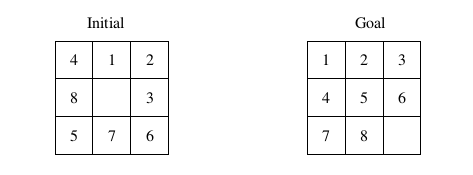
\includegraphics[scale=0.45]{images/image_initial_end}
\end{center}
\caption{The left tile$-$puzzle is the initial distribution of tiles and the right tile$-$puzzle is the goal distribution of tiles. Each one represent a State.} \label{fig:8tilepuzzle_begin}
\end{figure}


Instead of using an algorithm of Brute force search that will analyze all the possible solutions. We can obtain heuristics from the problem of the slide tile puzzle that will help us to solve the problem.

\section{Heuristics}
State$-$space algorithms, such as A* \cite{hart1968formal}, are important in many \texttt{AI} applications. A* uses the $f(s) = g(s) + h(s)$ cost function to guide its search. Here, $g(s)$ is the cost of the path from the start state $s$, and $h(s)$ is the estimated cost$-$to$-$go from $s$ to a gial; $h(.)$ is known as the heuristic function. The heuristic is the mathematical concept that represent to the estimate distance from the node $s$ to the nearest goal state.

\begin{figure}[htb]
\begin{center}
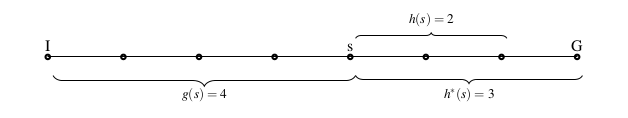
\includegraphics[scale=0.45]{images/image_search_tree}
\end{center}
\caption{Heuristic Search: \textit{I}: Initial State, \textit{s}: Some Sate, \textit{G}: Goal State} \label{fig:searchSpace}
\end{figure}

In the figure \ref{fig:searchSpace} the optimal distance from the Initial State $I$ to  the state $s$ is 4 and represented by $g(s)$. The $h\sp{*}(s)$ represent the optimal distance from $s$ to the Goal State $G$. And the $h(s)$ is the estimation distance from $s$ to $G$.

A heuristic function $h(s)$ estimates the cost of a solution path from $s$ to a goal state. A heuristic is admissible if $h(s) \leq h\sp{*}(s)$ for all $s \in V$, where $h\sp{*}(s)$ is the optimal cost of $s$. A heuristic is consisten iff $h(s) \leq c(s,t) + h(t)$ for all states $s$ and $t$, where $c(s,t)$ is the cost of the cheapest path from $s$ to $t$. For example, the heuristic function provided by a pattern database (\texttt{PDB}) heuristic \cite{culberson1998pattern} is admissible and consistent.

Given a set of admissible and consistent heuristics $\zeta = \{h_{1}, h_{2}, \dots, h_{M}\}$, the heuristic $h_{max}(s,\zeta) = $max$_{h \in \zeta} h(s)$ is also admissible and consistent. When describing our method we assume all heuristics to be consistent. We define $f_{max}(s, \zeta) = g(s) + h_{max}(s, \zeta)$, where $g(s)$ is the cost of the path expanded from $I$ to $s$. $g(s)$ is minimal when A$\sp{*}$ using a consistent heuristic expands $s$. We call an A$\sp{*}$ search tree the tree defined by the states expanded by A$\sp{*}$ using a consistent heuristic while solving a problem $\triangledown$.

\section{Problem Formulation}
When solving $\triangledown$ using the consistent heuristic function $h_{max}(\zeta\sp{'})$ for $\zeta\sp{'} \subseteq \zeta$, A$\sp{*}$ expands in the worst case $J(\zeta\sp{'}, \triangledown)$ nodes, where

\begin{equation}
J(\zeta\sp{'},\triangledown) = |\{s \in V | f_{max}(s,\zeta\sp{'} \leq C\sp{*})\}|
\label{eq:eq_size_search_tree_1}
\end{equation}

\begin{equation}
J(\zeta\sp{'},\triangledown) = |\{s \in V | h_{max}(s,\zeta\sp{'} \leq C\sp{*}) - g(s)\}|
\label{eq:eq_size_search_tree_2}
\end{equation}

We present a greedy algorithm for approximately solving the following optimization problem,

\begin{equation}
\begin{split}
\textbf{minimize}_{\zeta\sp{'} \in 2\sp{|\zeta|}}J(\zeta\sp{'}, \triangledown) \\
\textbf{subject to} |\zeta\sp{'} = N|
\end{split}
\end{equation}

Where $N$ could be determined by a hard constraint such as the maximum number of \texttt{PDBs} one can store in memory.

The heuristics can be obtained from each state of the problem. For example, for the problem of the 8$-$tile$-$puzzle figure \ref{fig:8tilepuzzle_begin} we can get two heuristics.

\subsection{Out of place (O.P)}
Counts the number of objects out of place.

\begin{figure}[htb]
\begin{center}
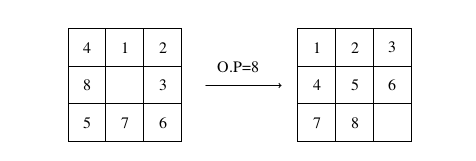
\includegraphics[scale=0.45]{images/image_op}
\end{center}
\caption{Out of place heuristic} \label{fig:8tilepuzzle_oop}
\end{figure}

The tiles numbered with 4, 1, 2, 3, 6, 7, 5, 8, and 4 are out of place then each object count as 1 and the sum would be 8.

\subsection{Manhatham Distance (M.D)}
Counts the minimum number of operations to get to the goal state.

\begin{figure}[htb]
\begin{center}
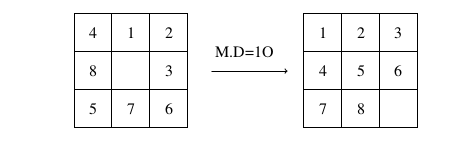
\includegraphics[scale=0.45]{images/image_md}
\end{center}
\caption{Manhatham distance heuristic} \label{fig:8tilepuzzle_md}
\end{figure}

The tile 4 count 1 to get to the goal position.
The tile 1 count 1 to get to the goal position.
The tile 2 count 1 to get to the goal position.
The tile 3 count 1 to get to the goal position.
The tile 6 count 1 to get to the goal position.
The tile 7 count 1 to get to the goal position.
The tile 5 count 1 to get to the goal position.
The tile 8 count 1 to get to the goal position.
Then the sum would be 10.

In order to solve the problem, we get the heuristics, which are information from the problem to solve the problem. Exists systems that can create heuristics for each problem. Those systems are called Heuristic Generators.

\section{Heuristic Generators}
Heuristic Generators works by creating abstractions of the original problem spaces.  There are different ways to abstract the problem space such as:

\subsection{Pattern Database (PDB)}
It's obtained by abstracting away certain problem variables, so that the remaining problem ("pattern") is small enough to be solved optimally for every state by blind exhaustive search. The results stored in a table, represent a PDB for the original problem. The abstraction of the search space gives an admissible heuristic function, mapping states to lower bounds.

\subsection{Neural Network}


\subsection{Genetic Algorithm}



\section{Take advantage of Heuristics}
The heuristics generators can create hundreds or even thousand of heuristics. In fact, exists different ways to take advantage of those heuristics. For example: If we want to use all the heuristics created by the heuristic generator. It would not be a good idea to use all of them because the main problem involved would be the time to evaluate each heuristic in the search tree, it could take too much time. \\

One way to take advantage of heuristics would be to take the maximum of the set of heuristics. For example, using three different heuristics $h1, h2$ and max($h1, h2$). Heuristic $h1$ and $h2$ are based on domain abstractions and the max($h1, h2$) is the maximum heuristic value of $h1$ and $h2$. \\

Exists different approaches to take advantage from a large set of heuristics. In this dissertation we use the meta$-$reasoning based on the minimum evaluation time. \\


\section{Number of heuristics to create.}
Something here

\begin{figure}[!htb]
\minipage{0.32\textwidth}
  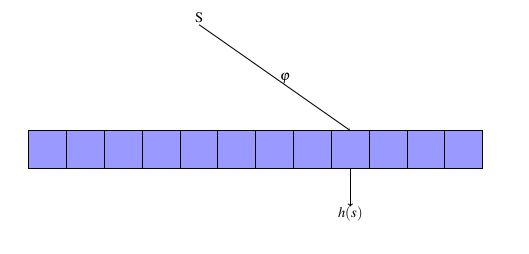
\includegraphics[width=\linewidth]{images/image_1_mem}
  \caption{One heuristic of size M}\label{fig:image1mem}
\endminipage\hfill
\minipage{0.32\textwidth}
  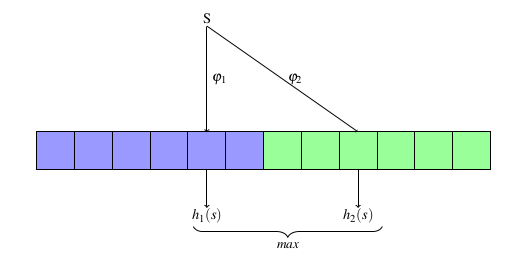
\includegraphics[width=\linewidth]{images/image_2_mem}
  \caption{Two heuristics of size M/2}\label{fig:image2mem}
\endminipage\hfill
\minipage{0.32\textwidth}%
  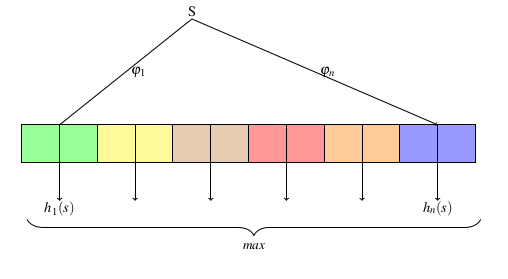
\includegraphics[width=\linewidth]{images/image_n_mem}
  \caption{N heuristics of size M/N}\label{fig:image3mem}
\endminipage
\end{figure}



\section{Heuristic Subset}
The heuristics generators systems can create many heuristics. Let's suppose $|\zeta| = $ 1000 heuristics were created considering the time and memory avaiable and we want to select the best N $=$ 100 heuristics. This would be: $${1000\choose 100} = 10\sp{138} possibilities$$
So, try to select heuristics from a large set of heuristics are going to be treated as an optimization problem. In order to select a subset of heuristics, our objective function should guarantee two properties: Monotonicity and Submodularity. \\





\normalsize

\section{---}
\noindent

\subsection{---}
\noindent

 \bigskip

In the next chapter, ... \\

\clearpage